Целью работы в текущем семестре стало написание программного модуля, осуществляющего поиск в ОС Windows (XP, 7, 8) следов установленных или удаленных программ. При этом реестр и директорию меню «Пуск» учитывать было не нужно.

\subsubsection{Директории в ОС, где программы могут оставить след}

В любой версии Windows (XP, 7, 8) необходимые директории:

\begin{enumerate}
  \item Program Files (рис.~\ref{kucher_1:kucher_1});
  \item Program Files (x86) (рис.~\ref{kucher_2:kucher_2});
  \item Program Files\textbackslash Common Files (рис.~\ref{kucher_3:kucher_3});
  \item Program Files (x86)\textbackslash Common Files (рис.~\ref{kucher_4:kucher_4}).
\end{enumerate}

\begin{figure}[h!]
\center{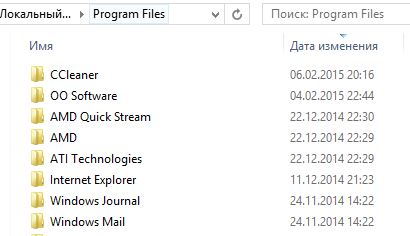
\includegraphics[width=0.4\linewidth]{kucher_1}}
\caption{Директория Program Files}
\label{kucher_1:kucher_1}
\end{figure} 

\begin{figure}[h!]
\center{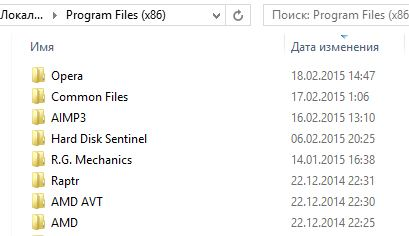
\includegraphics[width=0.4\linewidth]{kucher_2}}
\caption{Директория Program Files (x86)}
\label{kucher_2:kucher_2}
\end{figure} 

\begin{figure}[h!]
\center{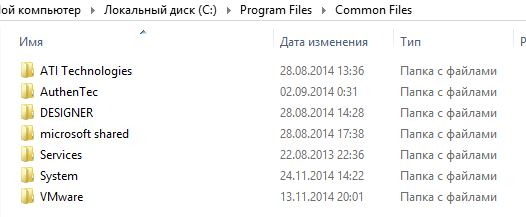
\includegraphics[width=0.7\linewidth]{kucher_3}}
\caption{Директория Program Files\textbackslash Common Files}
\label{kucher_3:kucher_3}
\end{figure} 

\begin{figure}[h!]
\center{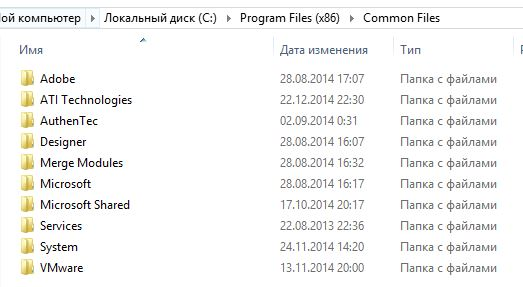
\includegraphics[width=0.6\linewidth]{kucher_4}}
\caption{Директория Program Files (x86)\textbackslash Common Files}
\label{kucher_4:kucher_4}
\end{figure} 


Далее расположение остаточных файлов зависит от OC.

Для Windows 7, 8:

\begin{enumerate}
  \item C:\textbackslash ProgramData (рис.~\ref{kucher_5:kucher_5});
  \item C:\textbackslash Users\textbackslash Имя пользователя\textbackslash AppData\textbackslash Local (рис.~\ref{kucher_6:kucher_6});
  \item C:\textbackslash Users\textbackslash Имя пользователя\textbackslash AppData\textbackslash Roaming (рис.~\ref{kucher_7:kucher_7});
  \item C:\textbackslash Users\textbackslash Default\textbackslash AppData\textbackslash Local;
  \item C:\textbackslash Users\textbackslash Default\textbackslash AppData\textbackslash Roaming.
\end{enumerate}

Для Windows XP:

\begin{enumerate}
  \item C:\textbackslash Documents and Settings\textbackslash Имя пользователя\textbackslash Application Data (рис.~\ref{kucher_8:kucher_8});
  \item C:\textbackslash Documents and Settings\textbackslash Имя пользователя\textbackslash LocalSettings\textbackslash ApplicationData;
\end{enumerate}

\begin{figure}[h!]
\center{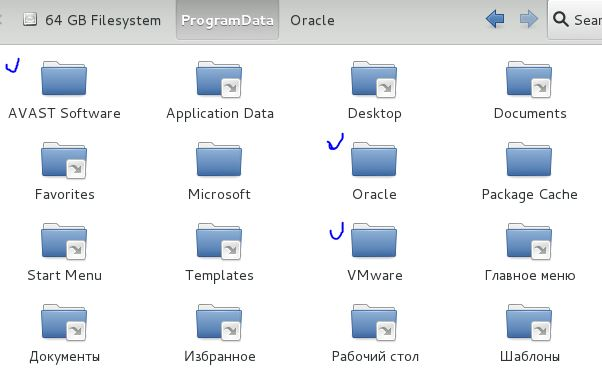
\includegraphics[width=0.6\linewidth]{kucher_5}}
\caption{Директория ProgramData}
\label{kucher_5:kucher_5}
\end{figure} 

\begin{figure}[h!]
\center{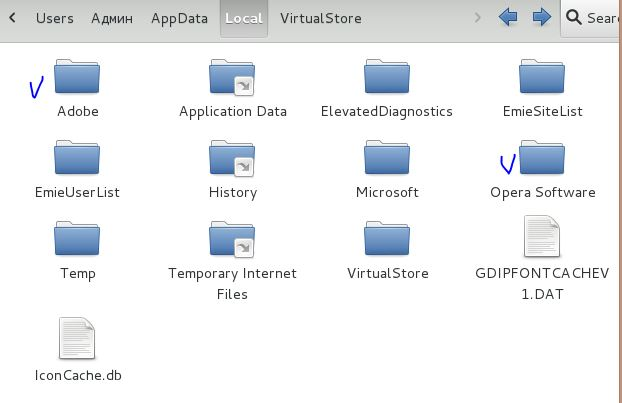
\includegraphics[width=0.6\linewidth]{kucher_6}}
\caption{Директория Local}
\label{kucher_6:kucher_6}
\end{figure} 

\begin{figure}[h!]
\center{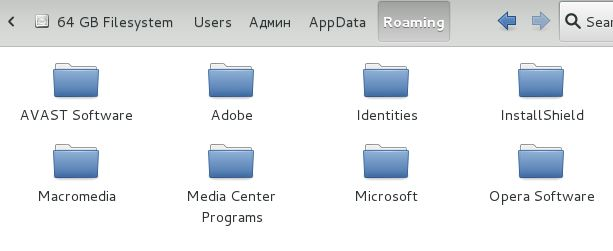
\includegraphics[width=0.6\linewidth]{kucher_7}}
\caption{Директория Roaming}
\label{kucher_7:kucher_7}
\end{figure} 

\begin{figure}[h!]
\center{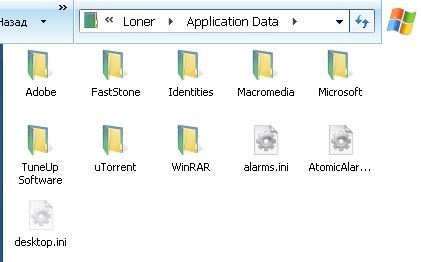
\includegraphics[width=0.6\linewidth]{kucher_8}}
\caption{Директория Application Data}
\label{kucher_8:kucher_8}
\end{figure} 

\clearpage
\subsubsection{Список эталонных каталогов для Windows XP x32}
\noindent C:\textbackslash Documents and Settings\textbackslash admin\textbackslash Application Data\textbackslash Identities \\
C:\textbackslash Documents and Settings\textbackslash admin\textbackslash Application Data\textbackslash Microsoft \\
C:\textbackslash Documents and Settings\textbackslash admin\textbackslash Local Settings\textbackslash Application Data\textbackslash Microsoft \\
C:\textbackslash Documents and Settings\textbackslash All Users\textbackslash Application Data\textbackslash Microsoft \\
C:\textbackslash Documents and Settings\textbackslash Default User\textbackslash Application Data\textbackslash Microsoft \\
C:\textbackslash Documents and Settings\textbackslash Default User\textbackslash Local Settings\textbackslash Application Data\textbackslash Microsoft \\
C:\textbackslash Program Files\textbackslash Common Files \\
C:\textbackslash Program Files\textbackslash ComPlus Applications \\
C:\textbackslash Program Files\textbackslash Internet Explorer \\
C:\textbackslash Program Files\textbackslash Messenger \\
C:\textbackslash Program Files\textbackslash microsoft frontpage \\
C:\textbackslash Program Files\textbackslash Movie Maker \\
C:\textbackslash Program Files\textbackslash MSN Gaming Zone \\
C:\textbackslash Program Files\textbackslash NetMeeting \\
C:\textbackslash Program Files\textbackslash Online Services \\
C:\textbackslash Program Files\textbackslash Outlook Express \\
C:\textbackslash Program Files\textbackslash Uninstall Information \\
C:\textbackslash Program Files\textbackslash Windows Media Player \\
C:\textbackslash Program Files\textbackslash Windows NT \\
C:\textbackslash Program Files\textbackslash WindowsUpdate \\
C:\textbackslash Program Files\textbackslash xerox \\
C:\textbackslash Program Files\textbackslash Common Files\textbackslash Microsoft Shared \\
C:\textbackslash Program Files\textbackslash Common Files\textbackslash MSSoap \\
C:\textbackslash Program Files\textbackslash Common Files\textbackslash ODBC \\
C:\textbackslash Program Files\textbackslash Common Files\textbackslash Services \\
C:\textbackslash Program Files\textbackslash Common Files\textbackslash SpeechEngines \\
C:\textbackslash Program Files\textbackslash Common Files\textbackslash System \\


\subsubsection{Список эталонных каталогов для Windows XP x64}
\noindent C:\textbackslash Documents and Settings\textbackslash Administrator\textbackslash Application Data\textbackslash Identities \\
C:\textbackslash Documents and Settings\textbackslash Administrator\textbackslash Application Data\textbackslash Microsoft \\
C:\textbackslash Documents and Settings\textbackslash Administrator\textbackslash Local Settings\textbackslash Application Data\textbackslash Microsoft \\
C:\textbackslash Documents and Settings\textbackslash All Users\textbackslash Application Data\textbackslash Microsoft \\
C:\textbackslash Documents and Settings\textbackslash Default User\textbackslash Application Data\textbackslash Microsoft \\
C:\textbackslash Documents and Settings\textbackslash Default User\textbackslash Local Settings\textbackslash Application Data\textbackslash Microsoft \\
C:\textbackslash Program Files\textbackslash Common Files \\
C:\textbackslash Program Files\textbackslash ComPlus Applications \\
C:\textbackslash Program Files\textbackslash Internet Explorer \\
C:\textbackslash Program Files\textbackslash Messenger \\
C:\textbackslash Program Files\textbackslash Online Services \\
C:\textbackslash Program Files\textbackslash Outlook Express \\
C:\textbackslash Program Files\textbackslash Windows NT \\
C:\textbackslash Program Files\textbackslash Common Files\textbackslash Microsoft Shared \\
C:\textbackslash Program Files\textbackslash Common Files\textbackslash ODBC \\
C:\textbackslash Program Files\textbackslash Common Files\textbackslash Services \\
C:\textbackslash Program Files\textbackslash Common Files\textbackslash SpeechEngines \\
C:\textbackslash Program Files\textbackslash Common Files\textbackslash System \\
C:\textbackslash Program Files (x86)\textbackslash Common Files \\
C:\textbackslash Program Files (x86)\textbackslash Internet Explorer \\
C:\textbackslash Program Files (x86)\textbackslash microsoft shared \\
C:\textbackslash Program Files (x86)\textbackslash Movie Maker \\
C:\textbackslash Program Files (x86)\textbackslash MSN \\
C:\textbackslash Program Files (x86)\textbackslash MSN Gaming Zone \\
C:\textbackslash Program Files (x86)\textbackslash NetMeeting \\
C:\textbackslash Program Files (x86)\textbackslash Outlook Express \\
C:\textbackslash Program Files (x86)\textbackslash speechengines \\
C:\textbackslash Program Files (x86)\textbackslash system \\
C:\textbackslash Program Files (x86)\textbackslash Uninstall Information \\
C:\textbackslash Program Files (x86)\textbackslash Windows Media Player \\
C:\textbackslash Program Files (x86)\textbackslash Windows Media Player[Strings] \\
C:\textbackslash Program Files (x86)\textbackslash Windows NT \\
C:\textbackslash Program Files (x86)\textbackslash Common Files\textbackslash Microsoft Shared \\
C:\textbackslash Program Files (x86)\textbackslash Common Files\textbackslash ODBC \\
C:\textbackslash Program Files (x86)\textbackslash Common Files\textbackslash Services \\
C:\textbackslash Program Files (x86)\textbackslash Common Files\textbackslash SpeechEngines \\
C:\textbackslash Program Files (x86)\textbackslash Common Files\textbackslash System \\


\subsubsection{Список эталонных каталогов для Windows 7 x32}
\noindent C:\textbackslash Program Files\textbackslash Common Files \\
C:\textbackslash Program Files\textbackslash DVD Maker \\
C:\textbackslash Program Files\textbackslash Internet Explorer \\
C:\textbackslash Program Files\textbackslash Microsoft Games \\
C:\textbackslash Program Files\textbackslash MSBuild \\
C:\textbackslash Program Files\textbackslash Reference Assemblies \\
C:\textbackslash Program Files\textbackslash Uninstall Information \\
C:\textbackslash Program Files\textbackslash Windows Defender \\
C:\textbackslash Program Files\textbackslash Windows Journal \\
C:\textbackslash Program Files\textbackslash Windows Mail \\
C:\textbackslash Program Files\textbackslash Windows Media Player \\
C:\textbackslash Program Files\textbackslash Windows NT \\
C:\textbackslash Program Files\textbackslash Windows Photo Viewer \\
C:\textbackslash Program Files\textbackslash Windows Portable Devices \\
C:\textbackslash Program Files\textbackslash Windows Sidebar \\
C:\textbackslash Program Files\textbackslash Common Files\textbackslash microsoft shared \\
C:\textbackslash Program Files\textbackslash Common Files\textbackslash Services \\
C:\textbackslash Program Files\textbackslash Common Files\textbackslash SpeechEngines \\
C:\textbackslash Program Files\textbackslash Common Files\textbackslash System \\
C:\textbackslash ProgramData\textbackslash Application Data \\
C:\textbackslash ProgramData\textbackslash Desktop \\
C:\textbackslash ProgramData\textbackslash Documents \\
C:\textbackslash ProgramData\textbackslash Favorites \\
C:\textbackslash ProgramData\textbackslash Microsoft \\
C:\textbackslash ProgramData\textbackslash Start Menu \\
C:\textbackslash ProgramData\textbackslash Templates \\
C:\textbackslash ProgramData\textbackslash Главное меню \\
C:\textbackslash ProgramData\textbackslash Документы \\
C:\textbackslash ProgramData\textbackslash Избранное \\
C:\textbackslash ProgramData\textbackslash Рабочий стол \\
C:\textbackslash ProgramData\textbackslash Шаблоны \\
C:\textbackslash Users\textbackslash admin\textbackslash AppData\textbackslash Local\textbackslash Application Data \\
C:\textbackslash Users\textbackslash admin\textbackslash AppData\textbackslash Local\textbackslash History \\
C:\textbackslash Users\textbackslash admin\textbackslash AppData\textbackslash Local\textbackslash Microsoft \\
C:\textbackslash Users\textbackslash admin\textbackslash AppData\textbackslash Local\textbackslash Temp \\
C:\textbackslash Users\textbackslash admin\textbackslash AppData\textbackslash Local\textbackslash Temporary Internet Files \\
C:\textbackslash Users\textbackslash admin\textbackslash AppData\textbackslash Local\textbackslash VirtualStore \\
C:\textbackslash Users\textbackslash admin\textbackslash AppData\textbackslash Roaming\textbackslash Identities \\
C:\textbackslash Users\textbackslash admin\textbackslash AppData\textbackslash Roaming\textbackslash Media Center Programs \\
C:\textbackslash Users\textbackslash admin\textbackslash AppData\textbackslash Roaming\textbackslash Microsoft \\
C:\textbackslash Users\textbackslash Default\textbackslash AppData\textbackslash Local\textbackslash Application Data \\
C:\textbackslash Users\textbackslash Default\textbackslash AppData\textbackslash Local\textbackslash History \\
C:\textbackslash Users\textbackslash Default\textbackslash AppData\textbackslash Local\textbackslash Microsoft \\
C:\textbackslash Users\textbackslash Default\textbackslash AppData\textbackslash Local\textbackslash Temp \\
C:\textbackslash Users\textbackslash Default\textbackslash AppData\textbackslash Local\textbackslash Temporary Internet Files \\
C:\textbackslash Users\textbackslash Default\textbackslash AppData\textbackslash Roaming\textbackslash Media Center Programs \\
C:\textbackslash Users\textbackslash Default\textbackslash AppData\textbackslash Roaming\textbackslash Microsoft \\


\subsubsection{Список эталонных каталогов для Windows 7 x64}
\noindent C:\textbackslash Program Files\textbackslash Common Files \\
C:\textbackslash Program Files\textbackslash DVD Maker \\
C:\textbackslash Program Files\textbackslash Internet Explorer \\
C:\textbackslash Program Files\textbackslash Microsoft Games \\
C:\textbackslash Program Files\textbackslash MSBuild \\
C:\textbackslash Program Files\textbackslash Reference Assemblies \\
C:\textbackslash Program Files\textbackslash Uninstall Information \\
C:\textbackslash Program Files\textbackslash Windows Defender \\
C:\textbackslash Program Files\textbackslash Windows Journal \\
C:\textbackslash Program Files\textbackslash Windows Mail \\
C:\textbackslash Program Files\textbackslash Windows Media Player \\
C:\textbackslash Program Files\textbackslash Windows NT \\
C:\textbackslash Program Files\textbackslash Windows Photo Viewer \\
C:\textbackslash Program Files\textbackslash Windows Portable Devices \\
C:\textbackslash Program Files\textbackslash Windows Sidebar \\
C:\textbackslash Program Files\textbackslash Common Files\textbackslash Microsoft Shared \\
C:\textbackslash Program Files\textbackslash Common Files\textbackslash Services \\
C:\textbackslash Program Files\textbackslash Common Files\textbackslash SpeechEngines \\
C:\textbackslash Program Files\textbackslash Common Files\textbackslash System \\
C:\textbackslash Program Files (x86)\textbackslash Common Files \\
C:\textbackslash Program Files (x86)\textbackslash Internet Explorer \\
C:\textbackslash Program Files (x86)\textbackslash MSBuild \\
C:\textbackslash Program Files (x86)\textbackslashReference Assemblies \\
C:\textbackslash Program Files (x86)\textbackslash Uninstall Information \\
C:\textbackslash Program Files (x86)\textbackslash Windows Defender \\
C:\textbackslash Program Files (x86)\textbackslash Windows Mail \\
C:\textbackslash Program Files (x86)\textbackslash Windows Media Player \\
C:\textbackslash Program Files (x86)\textbackslash Windows NT \\
C:\textbackslash Program Files (x86)\textbackslash Windows Photo Viewer \\
C:\textbackslash Program Files (x86)\textbackslash Windows Portable Devices \\
C:\textbackslash Program Files (x86)\textbackslash Windows Sidebar \\
C:\textbackslash Program Files (x86)\textbackslash Common Files\textbackslash microsoft shared \\
C:\textbackslash Program Files (x86)\textbackslash Common Files\textbackslash Services \\
C:\textbackslash Program Files (x86)\textbackslash Common Files\textbackslash SpeechEngines \\
C:\textbackslash Program Files (x86)\textbackslash Common Files\textbackslash System \\
C:\textbackslash ProgramData\textbackslash Application Data \\
C:\textbackslash ProgramData\textbackslash Desktop \\
C:\textbackslash ProgramData\textbackslash Documents \\
C:\textbackslash ProgramData\textbackslash Favorites \\
C:\textbackslash ProgramData\textbackslash Microsoft \\
C:\textbackslash ProgramData\textbackslash Start Menu \\
C:\textbackslash ProgramData\textbackslash Templates \\
C:\textbackslash ProgramData\textbackslash Главное меню \\
C:\textbackslash ProgramData\textbackslash Документы \\
C:\textbackslash ProgramData\textbackslash Избранное \\
C:\textbackslash ProgramData\textbackslash Рабочий стол \\
C:\textbackslash ProgramData\textbackslash Шаблоны \\
C:\textbackslash Users\textbackslash admin\textbackslash AppData\textbackslash Local\textbackslash Application Data \\
C:\textbackslash Users\textbackslash admin\textbackslash AppData\textbackslash Local\textbackslash History \\
C:\textbackslash Users\textbackslash admin\textbackslash AppData\textbackslash Local\textbackslash Microsoft \\
C:\textbackslash Users\textbackslash admin\textbackslash AppData\textbackslash Local\textbackslash Temp \\
C:\textbackslash Users\textbackslash admin\textbackslash AppData\textbackslash Local\textbackslash Temporary Internet Files \\
C:\textbackslash Users\textbackslash admin\textbackslash AppData\textbackslash Local\textbackslash VirtualStore \\
C:\textbackslash Users\textbackslash admin\textbackslash AppData\textbackslash Roaming\textbackslash Adobe \\
C:\textbackslash Users\textbackslash admin\textbackslash AppData\textbackslash Roaming\textbackslash Identities \\
C:\textbackslash Users\textbackslash admin\textbackslash AppData\textbackslash Roaming\textbackslash Media Center Programs \\
C:\textbackslash Users\textbackslash admin\textbackslash AppData\textbackslash Roaming\textbackslash Microsoft \\
C:\textbackslash Users\textbackslash Default\textbackslash AppData\textbackslash Local\textbackslash Application Data \\
C:\textbackslash Users\textbackslash Default\textbackslash AppData\textbackslash Local\textbackslash History \\
C:\textbackslash Users\textbackslash Default\textbackslash AppData\textbackslash Local\textbackslash Microsoft \\
C:\textbackslash Users\textbackslash Default\textbackslash AppData\textbackslash Local\textbackslash Temp \\
C:\textbackslash Users\textbackslash Default\textbackslash AppData\textbackslash Local\textbackslash Temporary Internet Files \\
C:\textbackslash Users\textbackslash Default\textbackslash AppData\textbackslash Roaming\textbackslash Media Center Programs \\
C:\textbackslash Users\textbackslash Default\textbackslash AppData\textbackslash Roaming\textbackslash Microsoft \\


\subsubsection{Список эталонных каталогов для Windows 8 x32}
\noindent C:\textbackslash Program Files\textbackslash Common Files \\
C:\textbackslash Program Files\textbackslash Embedded Lockdown Manager \\
C:\textbackslash Program Files\textbackslash Internet Explorer \\
C:\textbackslash Program Files\textbackslash Microsoft.NET \\
C:\textbackslash Program Files\textbackslash MSBuild \\
C:\textbackslash Program Files\textbackslash Reference Assemblies \\
C:\textbackslash Program Files\textbackslash Uninstall Information \\
C:\textbackslash Program Files\textbackslash Windows Defender \\
C:\textbackslash Program Files\textbackslash Windows Journal \\
C:\textbackslash Program Files\textbackslash Windows Mail \\
C:\textbackslash Program Files\textbackslash Windows Media Player \\
C:\textbackslash Program Files\textbackslash Windows Multimedia Platform \\
C:\textbackslash Program Files\textbackslash Windows NT \\
C:\textbackslash Program Files\textbackslash Windows Photo Viewer \\
C:\textbackslash Program Files\textbackslash Windows Portable Devices \\
C:\textbackslash Program Files\textbackslash Windows Sidebar \\
C:\textbackslash Program Files\textbackslash WindowsApps \\
C:\textbackslash Program Files\textbackslash WindowsPowerShell \\
C:\textbackslash Program Files\textbackslash Common Files\textbackslash microsoft shared \\
C:\textbackslash Program Files\textbackslash Common Files\textbackslash Services \\
C:\textbackslash Program Files\textbackslash Common Files\textbackslash System \\
C:\textbackslash ProgramData\textbackslash Application Data \\
C:\textbackslash ProgramData\textbackslash Desktop \\
C:\textbackslash ProgramData\textbackslash Documents \\
C:\textbackslash ProgramData\textbackslash Microsoft \\
C:\textbackslash ProgramData\textbackslash regid.1991-06.com.microsoft \\
C:\textbackslash ProgramData\textbackslash Start Menu \\
C:\textbackslash ProgramData\textbackslash Templates \\
C:\textbackslash ProgramData\textbackslash главное меню \\
C:\textbackslash ProgramData\textbackslash Документы \\
C:\textbackslash ProgramData\textbackslash Рабочий стол \\
C:\textbackslash ProgramData\textbackslash Шаблоны \\
C:\textbackslash Users\textbackslash admin\textbackslash AppData\textbackslash Local\textbackslash Application Data \\
C:\textbackslash Users\textbackslash admin\textbackslash AppData\textbackslash Local\textbackslash EmieBrowserModeList \\
C:\textbackslash Users\textbackslash admin\textbackslash AppData\textbackslash Local\textbackslash EmieSiteList \\
C:\textbackslash Users\textbackslash admin\textbackslash AppData\textbackslash Local\textbackslash EmieUserList \\
C:\textbackslash Users\textbackslash admin\textbackslash AppData\textbackslash Local\textbackslash History \\
C:\textbackslash Users\textbackslash admin\textbackslash AppData\textbackslash Local\textbackslash Microsoft \\
C:\textbackslash Users\textbackslash admin\textbackslash AppData\textbackslash Local\textbackslash Packages \\
C:\textbackslash Users\textbackslash admin\textbackslash AppData\textbackslash Local\textbackslash Temp \\
C:\textbackslash Users\textbackslash admin\textbackslash AppData\textbackslash Local\textbackslash Temporary Internet Files \\
C:\textbackslash Users\textbackslash admin\textbackslash AppData\textbackslash Local\textbackslash VirtualStore \\
C:\textbackslash Users\textbackslash admin\textbackslash AppData\textbackslash Roaming\textbackslash Adobe \\
C:\textbackslash Users\textbackslash admin\textbackslash AppData\textbackslash Roaming\textbackslash Microsoft \\
C:\textbackslash Users\textbackslash Default\textbackslash AppData\textbackslash Local\textbackslash Application Data \\
C:\textbackslash Users\textbackslash Default\textbackslash AppData\textbackslash Local\textbackslash History \\
C:\textbackslash Users\textbackslash Default\textbackslash AppData\textbackslash Local\textbackslash Microsoft \\
C:\textbackslash Users\textbackslash Default\textbackslash AppData\textbackslash Local\textbackslash Temp \\
C:\textbackslash Users\textbackslash Default\textbackslash AppData\textbackslash Local\textbackslash Temporary Internet Files \\
C:\textbackslash Users\textbackslash Default\textbackslash AppData\textbackslash Roaming\textbackslash Microsoft \\


\subsubsection{Список эталонных каталогов для Windows 8 x64}
\noindent C:\textbackslash Program Files\textbackslash Common Files \\
C:\textbackslash Program Files\textbackslash Internet Explorer \\
C:\textbackslash Program Files\textbackslash MSBuild \\
C:\textbackslash Program Files\textbackslash Reference Assemblies \\
C:\textbackslash Program Files\textbackslash Uninstall Information \\
C:\textbackslash Program Files\textbackslash Windows Defender \\
C:\textbackslash Program Files\textbackslash Windows Journal \\
C:\textbackslash Program Files\textbackslash Windows Mail \\
C:\textbackslash Program Files\textbackslash Windows Media Player \\
C:\textbackslash Program Files\textbackslash Windows Multimedia Platform \\
C:\textbackslash Program Files\textbackslash Windows NT \\
C:\textbackslash Program Files\textbackslash Windows Photo Viewer \\
C:\textbackslash Program Files\textbackslash Windows Portable Devices \\
C:\textbackslash Program Files\textbackslash Windows Sidebar \\
C:\textbackslash Program Files\textbackslash WindowsApps \\
C:\textbackslash Program Files\textbackslash WindowsPowerShell \\
C:\textbackslash Program Files\textbackslash Common Files\textbackslash microsoft shared \\
C:\textbackslash Program Files\textbackslash Common Files\textbackslash Services \\
C:\textbackslash Program Files\textbackslash Common Files\textbackslash System \\
C:\textbackslash Program Files (x86)\textbackslash Common Files \\
C:\textbackslash Program Files (x86)\textbackslash Internet Explorer \\
C:\textbackslash Program Files (x86)\textbackslash Microsoft.NET \\
C:\textbackslash Program Files (x86)\textbackslash MSBuild \\
C:\textbackslash Program Files (x86)\textbackslash Reference Assemblies \\
C:\textbackslash Program Files (x86)\textbackslash Windows Defender \\
C:\textbackslash Program Files (x86)\textbackslash Windows Mail \\
C:\textbackslash Program Files (x86)\textbackslash Windows Media Player \\
C:\textbackslash Program Files (x86)\textbackslash Windows Multimedia Platform \\
C:\textbackslash Program Files (x86)\textbackslash Windows NT \\
C:\textbackslash Program Files (x86)\textbackslash Windows Photo Viewer \\
C:\textbackslash Program Files (x86)\textbackslash Windows Portable Devices \\
C:\textbackslash Program Files (x86)\textbackslash Windows Sidebar \\
C:\textbackslash Program Files (x86)\textbackslash WindowsPowerShell \\
C:\textbackslash Program Files (x86)\textbackslash Common Files\textbackslash Microsoft Shared \\
C:\textbackslash Program Files (x86)\textbackslash Common Files\textbackslash Services \\
C:\textbackslash Program Files (x86)\textbackslash Common Files\textbackslash System \\
C:\textbackslash ProgramData\textbackslash Application Data \\
C:\textbackslash ProgramData\textbackslash Desktop \\
C:\textbackslash ProgramData\textbackslash Documents \\
C:\textbackslash ProgramData\textbackslash Microsoft \\
C:\textbackslash ProgramData\textbackslash regid.1991-06.com.microsoft \\
C:\textbackslash ProgramData\textbackslash Start Menu \\
C:\textbackslash ProgramData\textbackslash Templates \\
C:\textbackslash ProgramData\textbackslash главное меню \\
C:\textbackslash ProgramData\textbackslash Документы \\
C:\textbackslash ProgramData\textbackslash Рабочий стол \\
C:\textbackslash ProgramData\textbackslash Шаблоны \\
C:\textbackslash Users\textbackslash agaerg\textbackslash AppData\textbackslash Local\textbackslash Application Data \\
C:\textbackslash Users\textbackslash agaerg\textbackslash AppData\textbackslash Local\textbackslash History \\
C:\textbackslash Users\textbackslash agaerg\textbackslash AppData\textbackslash Local\textbackslash Microsoft \\
C:\textbackslash Users\textbackslash agaerg\textbackslash AppData\textbackslash Local\textbackslash Packages \\
C:\textbackslash Users\textbackslash agaerg\textbackslash AppData\textbackslash Local\textbackslash Temp \\
C:\textbackslash Users\textbackslash agaerg\textbackslash AppData\textbackslash Local\textbackslash Temporary Internet Files \\
C:\textbackslash Users\textbackslash agaerg\textbackslash AppData\textbackslash Local\textbackslash VirtualStore \\
C:\textbackslash Users\textbackslash agaerg\textbackslash AppData\textbackslash Roaming\textbackslash Adobe \\
C:\textbackslash Users\textbackslash agaerg\textbackslash AppData\textbackslash Roaming\textbackslash Identities \\
C:\textbackslash Users\textbackslash agaerg\textbackslash AppData\textbackslash Roaming\textbackslash Microsoft \\
C:\textbackslash Users\textbackslash Default\textbackslash AppData\textbackslash Local\textbackslash Application Data \\
C:\textbackslash Users\textbackslash Default\textbackslash AppData\textbackslash Local\textbackslash History \\
C:\textbackslash Users\textbackslash Default\textbackslash AppData\textbackslash Local\textbackslash Microsoft \\
C:\textbackslash Users\textbackslash Default\textbackslash AppData\textbackslash Local\textbackslash Temp \\
C:\textbackslash Users\textbackslash Default\textbackslash AppData\textbackslash Local\textbackslash Temporary Internet Files \\
C:\textbackslash Users\textbackslash Default\textbackslash AppData\textbackslash Roaming\textbackslash Microsoft \\


\subsubsection{Блок-схема алгоритма работы программного модуля SearchProgram}

\begin{figure}[h!]
\center{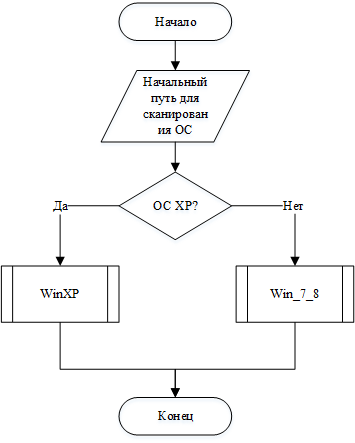
\includegraphics[width=0.5\linewidth]{kucher_9}}
\caption{Блок-схема основной программы}
\label{kucher_9:kucher_9}
\end{figure}

\begin{figure}[h!]
\center{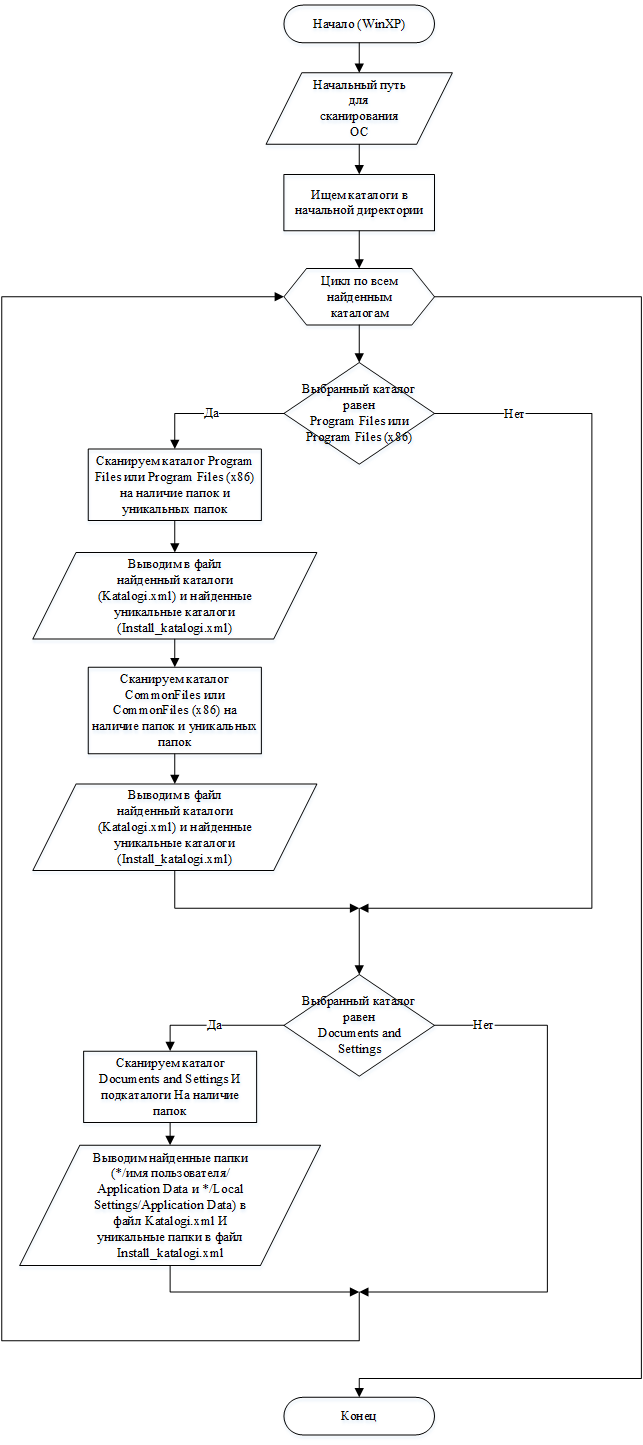
\includegraphics[width=0.6\linewidth]{kucher_10}}
\caption{Блок-схема функции WinXP}
\label{kucher_10:kucher_10}
\end{figure}

\begin{figure}[h!]
\center{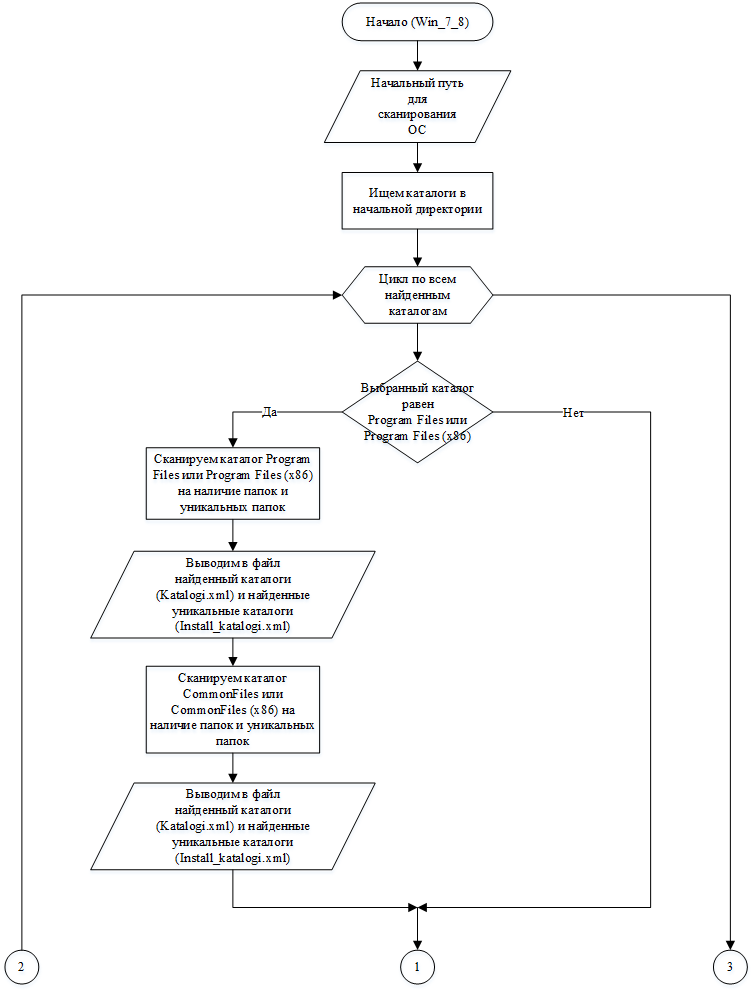
\includegraphics[width=0.8\linewidth]{kucher_11}}
\caption{Блок-схема функции Win\_7\_8}
\label{kucher_11:kucher_11}
\end{figure}

\begin{figure}[h!]
\center{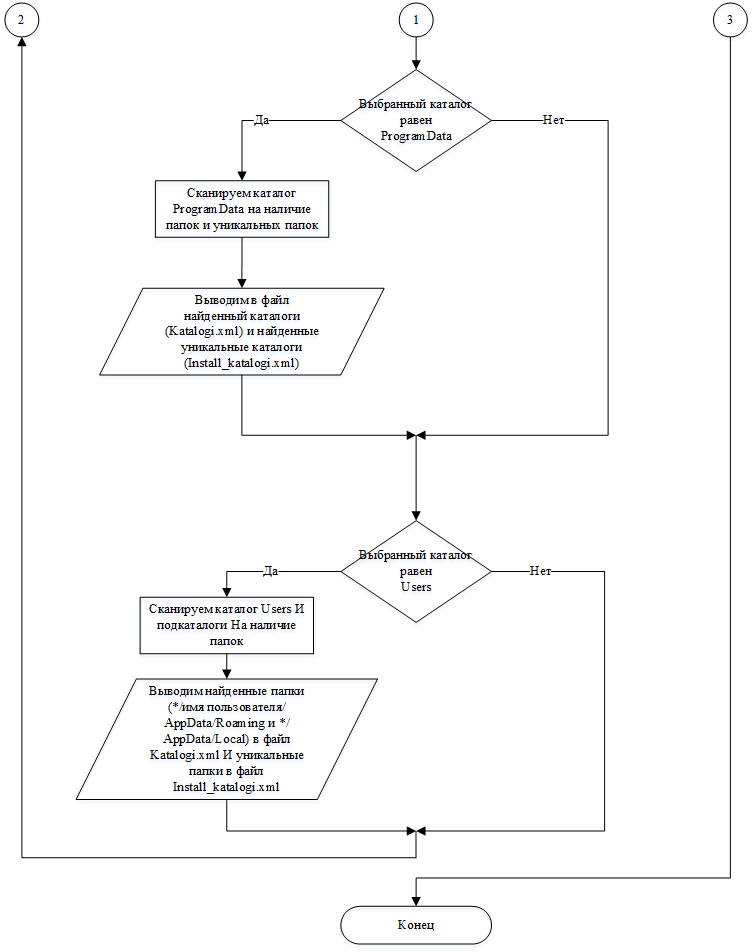
\includegraphics[width=0.8\linewidth]{kucher_18}}
\caption{Продолжение блок-схемы функции Win\_7\_8}
\label{kucher_18:kucher_18}
\end{figure}

\clearpage
\subsubsection{Описание плагина TaskSearchProgram}

Плагин TaskSearchProgram получает начальный путь, с которого он начнет сканировать ОС и путь для сохранения результатов. В зависимости от полученной ОС (на данный момент версия вводится вручную, в дальнейшем это будет автоматизировано) запускается либо функция <<WinXP>>, либо <<Win\_7\_8>>. Далее происходит сканирование каталогов и подкаталогов, вывод найденных директорий в файл <<katalogi.xml>>. Вдобавок, найденные директории сравниваются с шаблонами, собранными из <<чистых>> ОС. Те директории, которые не совпали с шаблонами, выводятся в отдельный файл <<install\_katalogi.xml>>. Плагин сканирует директории, указанные в предыдущих разделах.

Результаты работы плагина, записанные в выходные XML-файлы, можно увидеть на рисунках~\ref{kucher_12:kucher_12} ---~\ref{kucher_17:kucher_17}.

\begin{figure}[h!]
\center{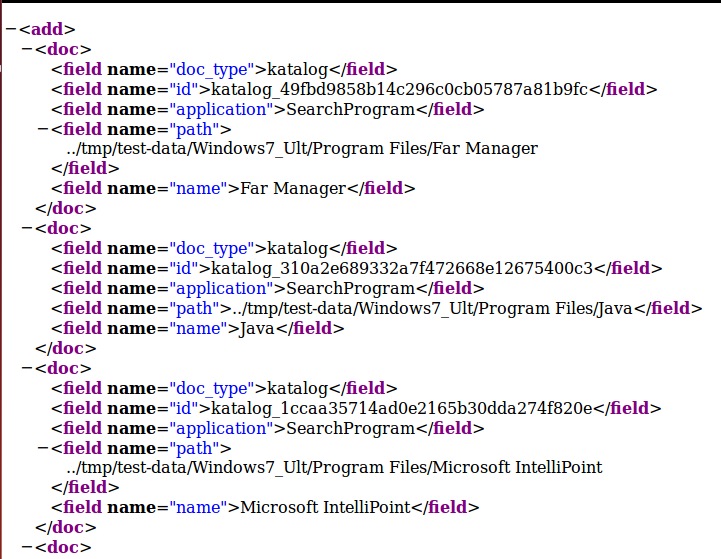
\includegraphics[width=0.5\linewidth]{kucher_12}}
\caption{Содержимое файла install\_katalogi.xml для Windows7}
\label{kucher_12:kucher_12}
\end{figure}

\begin{figure}[h!]
\center{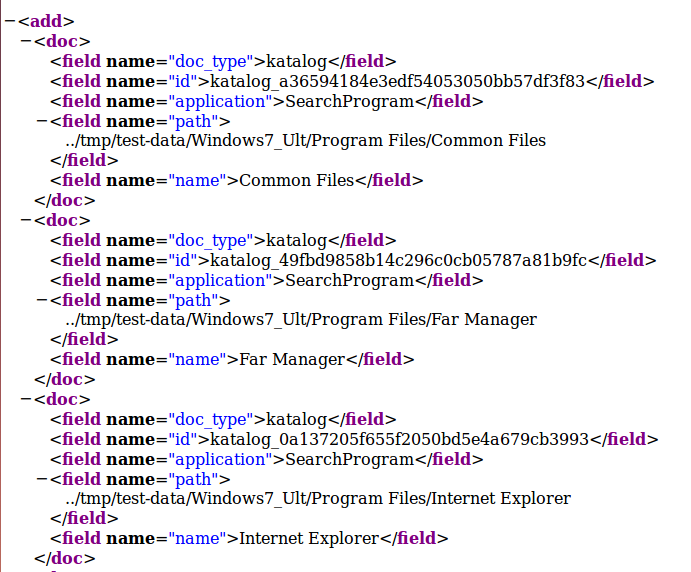
\includegraphics[width=0.5\linewidth]{kucher_13}}
\caption{Содержимое файла install.xml для Windows7}
\label{kucher_13:kucher_13}
\end{figure}

\begin{figure}[h!]
\center{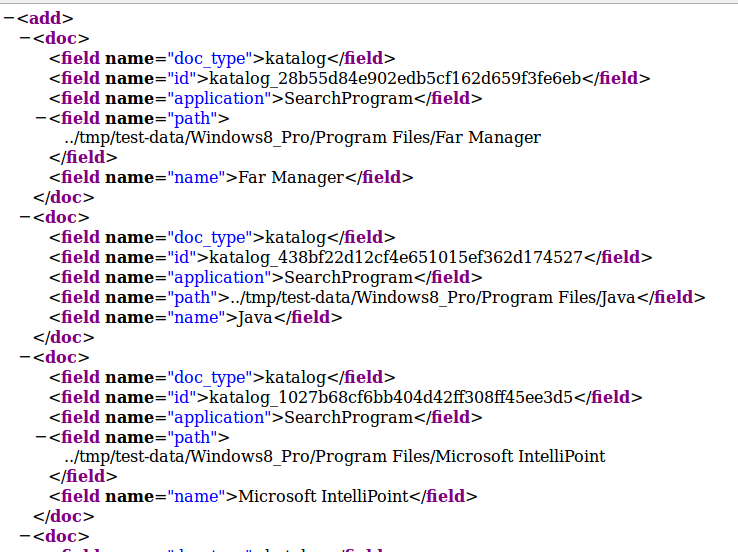
\includegraphics[width=0.5\linewidth]{kucher_14}}
\caption{Содержимое файла install\_katalogi.xml для Windows 8}
\label{kucher_14:kucher_14}
\end{figure}

\begin{figure}[h!]
\center{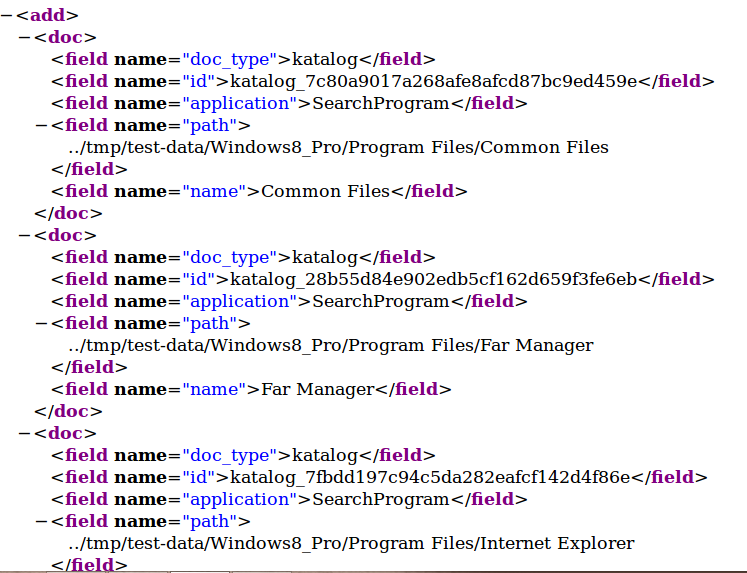
\includegraphics[width=0.5\linewidth]{kucher_15}}
\caption{Содержимое файла install.xml для Windows 8}
\label{kucher_15:kucher_15}
\end{figure}

\begin{figure}[h!]
\center{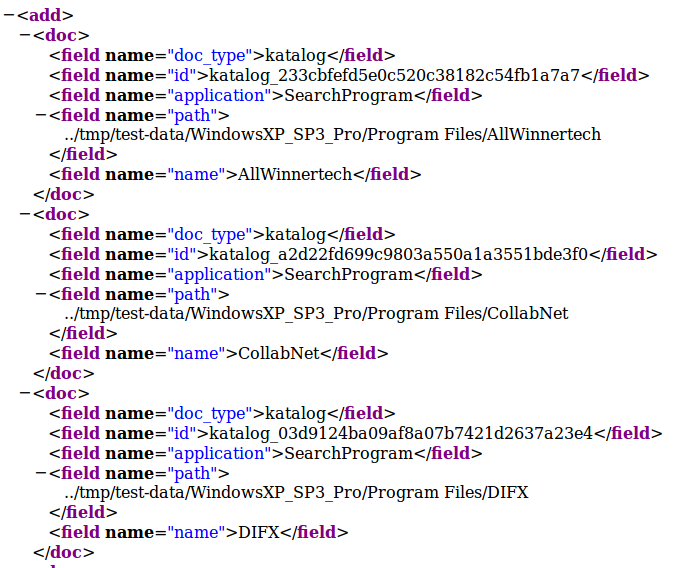
\includegraphics[width=0.5\linewidth]{kucher_16}}
\caption{Содержимое файла install\_katalogi.xml для Windows XP}
\label{kucher_16:kucher_16}
\end{figure}

\begin{figure}[h!]
\center{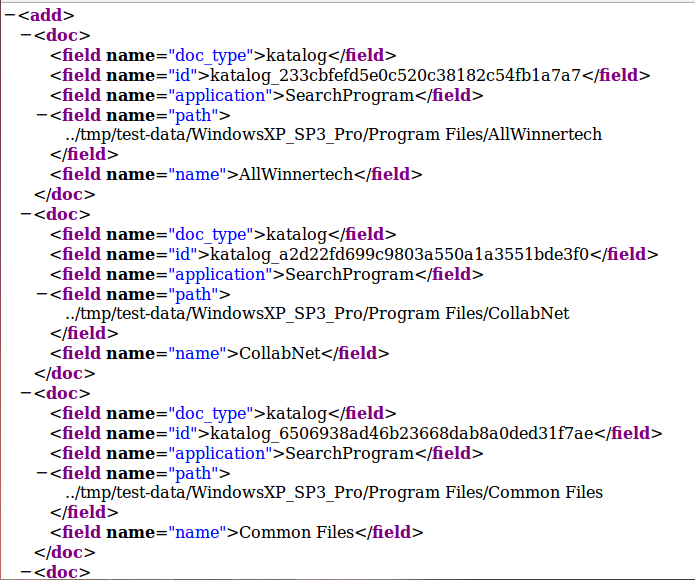
\includegraphics[width=0.8\linewidth]{kucher_17}}
\caption{Содержимое файла install.xml для Windows XP}
\label{kucher_17:kucher_17}
\end{figure}

\clearpage

